\documentclass[11pt]{article}


\usepackage[utf8]{inputenc}
\usepackage[T1]{fontenc}
\usepackage[french]{babel}
 
\usepackage{algorithm}
\usepackage{algorithmic}
\usepackage[T1]{fontenc}
\usepackage{enumitem}
\usepackage{hyperref}
\usepackage{graphicx}
\usepackage{color}
\usepackage{listings}
\usepackage{wrapfig}
\usepackage{amsfonts}
\usepackage{amsmath}
\usepackage{mathtools}
\usepackage[left=2cm,right=2cm,top=2cm,bottom=2cm]{geometry}
\usepackage{framed}
\usepackage{mathenv}
\usepackage{blkarray}
\usepackage{xcolor}
\usepackage{pdflscape}
% \usepackage[sfdefault]{FiraSans} %selon vos goûts et couleurs

\setlist[enumerate]{itemsep=5ex}

%extensions requises par bclogo
\usepackage{xkeyval}
\usepackage{ifthen}
\usepackage{ifpdf}
\usepackage{etoolbox}
\usepackage[tikz]{bclogo}

%paramètres de bclogo
\presetkeys{bclogo}{ombre=true,epOmbre=0.25}{}
\newcommand{\eb}{\end{bclogo}}

%paramétrage bclogo définition
\newcounter{definition}
\setcounter{definition}{0}
\newcommand{\bd}[1]{\addtocounter{definition}{1} \begin{bclogo}[logo=\bcinfo ,sousTitre=#1,nobreak=true]{Définition \thedefinition}}

%parametrage bclogo remarque
\newcommand{\br}{\begin{bclogo}[margeG=1,noborder=true,nobreak=true]{Remarque}}

%title setuplisting
\title{Projet de gestion de données avancée}
\author{Damien LU, Gabriel MÉZIÈRE, Louise DESSERT}

% table of contents setup
\renewcommand{\contentsname}{Sommaire}
\usepackage{etoolbox}
\patchcmd{\thebibliography}{\section*{\refname}}{}{}{}

% systeme d'équation
\newenvironment{sistema}%
{\left\lbrace\begin{array}{@{}l@{}}}%
  {\end{array}\right.}

\setlength{\parindent}{0cm}
\setlength{\parskip}{1ex plus 0.5ex minus 0.2ex}
\newcommand{\hsp}{\hspace{20pt}}
\newcommand{\HRule}{\rule{\linewidth}{0.5mm}}

\hypersetup{
  colorlinks,
  citecolor=black,
  filecolor=black,
  linkcolor=black,
  urlcolor=red
}

\lstset{basicstyle=\ttfamily,showstringspaces=false,breaklines=true, language=SQL,keywordstyle=\color{blue},commentstyle=\color{gray},breakindent=1.5em,
xleftmargin=2em,xrightmargin=2em,frame=single,rulecolor=\color{orange},
backgroundcolor=\color{yellow!5},columns=fullflexible}
\begin{document}

  \maketitle
  \tableofcontents
~\\ \hrule

\section{Objectifs du Projet}

L'objectif de ce projet est de mettre en application l'ensemble des notions vues en cours, via l'utilisation du logiciel Neo4j. Nous utiliserons la base de données CitationDB fournie dans le sujet qui met en relation des auteurs et des articles.


\section{Requêtes analytiques simples}

\begin{enumerate}
\item  
Voici le schéma que nous avons inferé
\begin{figure}[H]
  \centerline{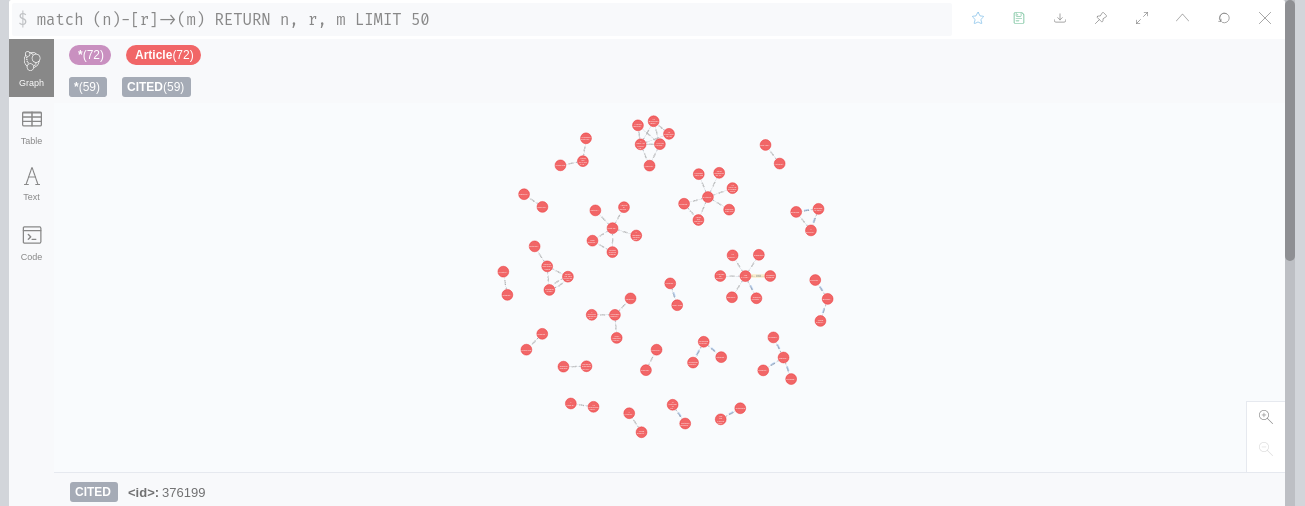
\includegraphics[scale=0.45]{schema_complet_rep.png}}
  \caption{Schéma du graphe limité à 50 noeuds}
\end{figure}
\item 
Pour trouver quel était le label le plus fréquent dans notre jeu
de données nous avons utilisé les requêtes suivantes pour comparer les différents labels :
\begin{lstlisting}
MATCH p = (n:Author) RETURN count(p)
MATCH p = (n:Article) RETURN count(p) 
MATCH p = (n:Venue) RETURN count(p)
\end{lstlisting}

Nous obtenons comme résultats, 81299 pour Author, 51956 pour Article et 4 pour Venue.
\textbf{Le label la plus fréquent est donc Author.}
\item 
Pour trouver le nombre moyen d'articles publiés par auteur nous avons utilisé la requête suivante :
\begin{lstlisting}
MATCH (n)-[q:AUTHOR]->(r) 
WITH r.name as g,count(n) as t 
RETURN avg(t)
\end{lstlisting}

Nous avons, grâce à ceci, pu observer que les auteurs de la base publiaient en moyenne 1.75 articles.
\item 
Nous avons utilisé la requête suivante pour trouver l'auteur qui avait publié le plus d'articles : 
\begin{lstlisting}
MATCH (n)-[q:AUTHOR]->(r) 
WITH r.name as nam,count(n) as ct 
WITH apoc.agg.maxItems(nam,ct) as maxData 
RETURN maxData.items, maxData.value
\end{lstlisting}
Ici, nous comptons le nombre d'articles par auteur puis récupérons ensuite le nombre le plus haut.

\textbf{Peter G. Neumann a publié le plus d'articles avec en tout, 89 ouvrages.}
\item 
Nous obtenons l'année dans laquelle le plus de publications sont apparues en utilisant la requête suivante :
\begin{lstlisting}
MATCH (n:Article) 
WITH n.year as date,count(n) as ct 
WITH apoc.agg.maxItems(date,ct) as maxdata 
RETURN maxdata.items, maxdata.value
\end{lstlisting}
Ici nous comptons le nombre de publications par année en prenant soin de conserver le titre de la publication associée à la valeur maximale.

\textbf{L'année recherchée est l'année 2006 avec en tout 7536 publications.}
\end{enumerate}

\section{Requêtes analytiques plus complexes}
\begin{enumerate}[resume]
\item 
Pour obtenir les 20 futurs collaborateurs les plus probables de Brian Fitzgerarld, l'idée est de d'abord chercher les auteurs qui ont publié au moins un article avec Brian Fitzgerald puis de chercher les co-auteurs de ces co-auteurs qui ne sont pas Brian Fitzgerald. Ainsi, nous proposons la requête ci-dessous :
\begin{lstlisting}
MATCH (t)<-[s:AUTHOR]-(n)-[q:AUTHOR]->(r) 
WHERE r.name = "Brian Fitzgerald" 
WITH collect(t.name) as l 
MATCH (a)<-[b:AUTHOR]-(c)-[d:AUTHOR]->(e) 
WHERE e in l and a.name <> "Brian Fitzgerald" 
RETURN collect(a.name)
\end{lstlisting}
Cette requête n'a pas abouti...
\item
Cette question dépend de la question 6 que nous n'avons pas réussi..
\item 
Nous avons ajouté, à chaque node Article, le PageRank correspondant à son influence par rapport aux relations CITED en suivant le canevas suivant :
\begin{itemize}
    \item créer une projection en mémoire du graphe :
    \begin{lstlisting}
CALL gds.graph.create('graph','Article',{ CITED: { orientation: 'UNDIRECTED'}})
    \end{lstlisting}
    \item puis écrire dans chaque noeud du graphe la propriété \texttt{pageRank} avec la procédure suivante :
    \begin{lstlisting}
CALL gds.pageRank.write('graph', {writeProperty: 'pageRank'})
    \end{lstlisting}
\end{itemize}
\textbf{Tous les noeuds Article contiennent désormais un champ supplémentaire pageRank.}
\item 
Nous avons calculé les articles les plus influents en fonction de la mesure PageRank que nous avions mis en place précedemment.
\begin{lstlisting}
MATCH (n:Article) RETURN n.title,n.pageRank ORDER BY n.pageRank DESC LIMIT 10
\end{lstlisting}
La requête précédente, nous a permis d'obtenir le résultat suivant :
\begin{figure}[H]
    \centerline{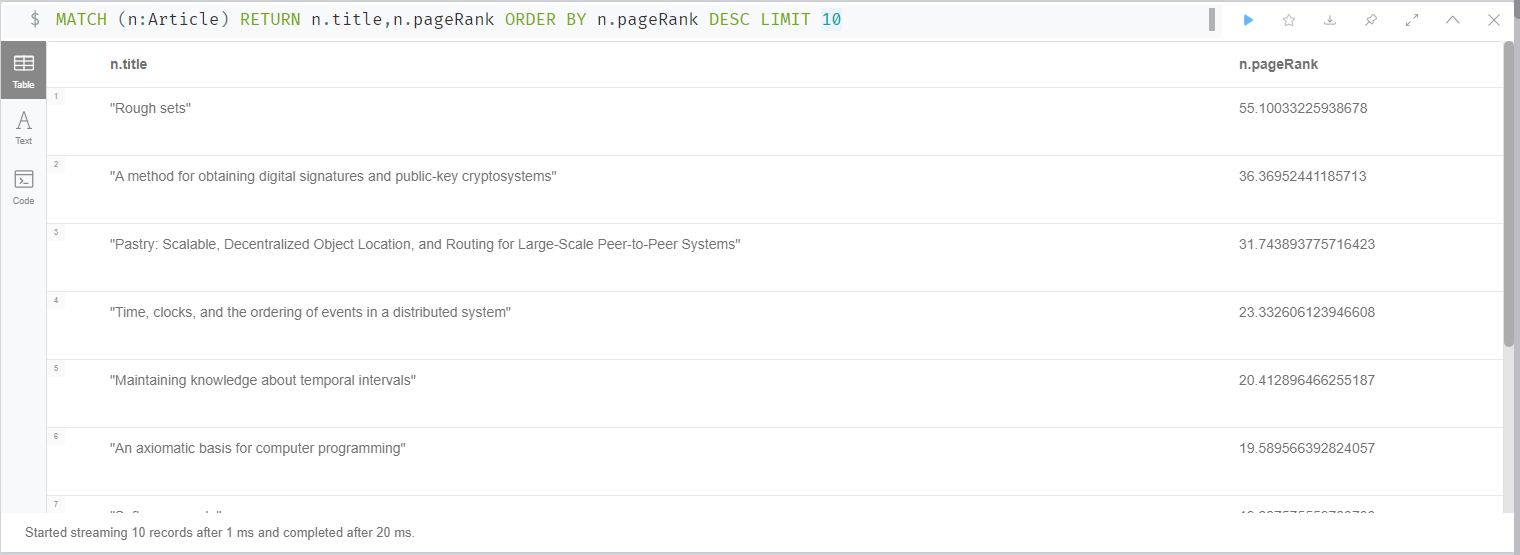
\includegraphics[scale=0.5]{q9.PNG}}
    \caption{Sélection des 10 articles les plus influents selon la mesure PageRank}
\end{figure}
\item 
Nous avons créé un index sur les propriétés 'title' et 'abstract' avec la requête fournie par l'énoncé et vérifié que ce dernier était correct.

Puis, nous avons cherché à trouver dans cet index, les auteurs qui ont publié le plus d'articles opensource, en effectuant la requête suivante :
\begin{lstlisting}
CALL db.index.fulltext.queryNodes("articles", "open source") YIELD node 
WITH [(author)<-[:AUTHOR]-(node) | author.name] as tab 
UNWIND tab as t 
WITH collect(t) as list 
WITH apoc.coll.frequencies(list) AS res 
RETURN apoc.coll.sortMaps(res,"count")
\end{lstlisting}
\textbf{Denys Poshyvanyk remporte ce "titre" avec 16 publications.}
\item 
Nous avons créé un index de recherche pour la propriété name des noeuds avec le label Authors de la manière suivante :
\begin{lstlisting}
CREATE index on :Authors(name)
\end{lstlisting}
\item 
Notre objectif est de créer une relation CO\_AUTHOR qui permet de relier chaque deux auteurs qui ont collaboré sur au moins un article. Nous suivrons le canevas suivant :
\begin{itemize}
    \item on recherche tous les couples d'auteurs qui ont publié au moins un article en commun. On crée alors une relation entre ces auteurs du type CO\_AUTHOR (sans spécifier pour l'instant de propriétés - nous le ferons plus tard)
    \begin{lstlisting}
MATCH (d)<-[e:AUTHOR]-(a)-[b:AUTHOR]->(c) CREATE UNIQUE (d)-[t:CO_AUTHOR]->(c) RETURN type(t)
    \end{lstlisting}
    \item on ajoute ensuite les propriétés year et collaborations aux relations CO\_AUTHOR avec la requête suivante :
    \begin{lstlisting}
MATCH (a)-[t:CO_AUTHOR]->(b) 
    # le minimum de la liste des annees de publication des articles
SET t.year = apoc.coll.min([(a)<-[r:AUTHOR]-(s)-[v:AUTHOR]->(b) | s.year])
    # la longueur de la liste des articles ecrits en collaboration entre les auteurs a et b
SET t.collaborations = size([(a)<-[r:AUTHOR]-(s)-[v:AUTHOR]->(b) | s.year])
RETURN a.name,b.name,t.year,t.collaborations
    \end{lstlisting}
\end{itemize}
\item 
Nous avons crée des nouvelles relations CO-AUTHOR-EARLY et CO-AUTHOR-LATE entre des nœuds, correspondant à des co-auteurs qui ont été publiés ensemble respectivement avant et après 2006 : pour cela, il suffit de regarder la propriété year des relations CO\_AUTHOR et de filtrer selon si l'année est inférieure à 2006 ou non :
\begin{lstlisting}
MATCH (a)-[t:CO_AUTHOR]->(b) WHERE t.year<2006 CREATE (a)-[s:CO_AUTHOR_EARLY]->(b) RETURN a.name,b.name,type(s)
MATCH (a)-[t:CO_AUTHOR]->(b) WHERE t.year>=2006 CREATE (a)-[s:CO_AUTHOR_LATE]->(b) RETURN a.name,b.name,type(s)
\end{lstlisting}
\end{enumerate}

\section{Requêtes analytiques avec applications d'algorithmes}

\begin{enumerate}[resume]
\item 
Avec la requête fournie, on crée une projection en mémoire du graphe, qu'on appelle dans la suite \texttt{whole-graph}. Cette projection qui servira dans toute la suite permet de pouvoir appliquer les différents algorithmes de recherche directement sur ce graphe en mémoire. En effet, on exécute ensuite l'algorithme de comptage des triangles, qui est fourni dans la bilbiothèque gds sur les relations CO\_AUTHOR\_EARLY et CO\_AUTHOR\_LATE. Cet algorithme renvoie le nombre de triangles, c'est-à-dire le nombre de cliques de taille 3 et écrit dans les noeuds du graphe reliés par une relation CO\_AUTHOR\_EARLY ou CO\_AUTHOR\_LATE la propriété triangles pour déterminer l'appartenance à un triangle $i$ d'un noeud. Cet algorithme prend alors la forme de la requête suivante :
\begin{lstlisting}
CALL gds.alpha.triangleCount.write('whole-graph', {relationshipTypes:['CO_AUTHOR_EARLY'],
  writeProperty: 'triangles', clusteringCoefficientProperty:'clustering'
}) YIELD nodeCount, triangleCount, averageClusteringCoefficient

CALL gds.alpha.triangleCount.write('whole-graph', {relationshipTypes:['CO_AUTHOR_LATE'],
  writeProperty: 'triangles', clusteringCoefficientProperty:'clustering'
}) YIELD nodeCount, triangleCount, averageClusteringCoefficient
\end{lstlisting}
Les résultats obtenus sont le nombre de triangles dans le graphe avec les deux types de relation : on en déduit le le calcul du coefficient de clustering global pour chacune des deux relations en fonction du nombre de triangles obtenu précédemment. On obtient les résultats suivants :

\begin{figure}[H]
    \centerline{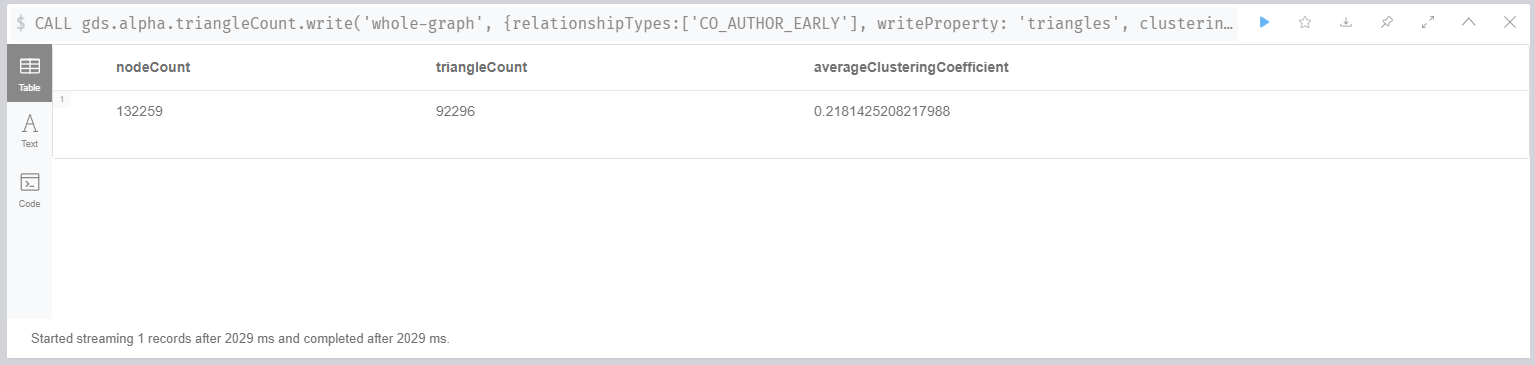
\includegraphics[scale=0.5]{q14a.PNG}}
    \centerline{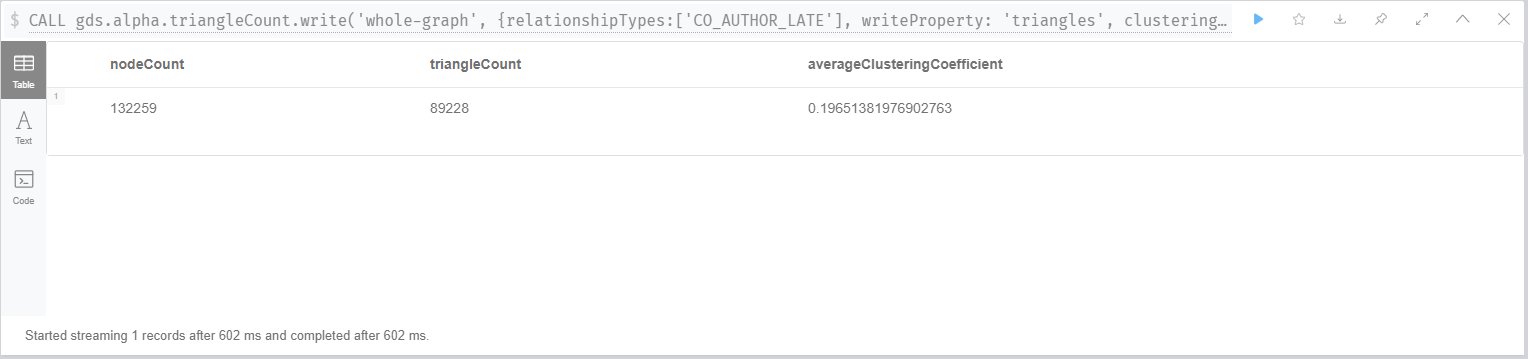
\includegraphics[scale=0.5]{q14b.PNG}}
    \caption{Résultat de l'algorithme de comptage des triangles et calcul du coefficient de clustering}
\end{figure}

Le coefficient de clustering calculé ici est global et représente la probabilité que deux auteurs distincts ayant un coauteur en commun soient eux-mêmes coauteurs. Il est défini de la manière suivante :
\bd{Coefficient de clustering global}
Le coefficient de clustering global d'un graphe est la quantité $C$, définie par :
$$ C = \dfrac{3\times \text{card}(\text{triangles})}{\text{card}(\text{paires de voisins distincts d'un noeud de degré d})} $$
\eb
Le coefficient de clustering valant respectivement 0.2181425208217988 et 0.19651381976902763, et étant dans les deux cas largement inférieur à 1, \textbf{"les collaborateurs de mes collaborateurs ne sont pas susceptibles d'être mes collaborateurs"}.
\item 
Cette fois-ci, on utilise l'algorithme de recherche des composantes connexes du graphe, sur la relation CITED. La requête est alors :
\begin{lstlisting}
CALL gds.alpha.scc.write('whole-graph', {relationshipTypes: ['CITED'], writeProperty: 'componentId'})
YIELD setCount, maxSetSize, minSetSize
\end{lstlisting}
L'algorithme écrit alors sur tous les noeuds étant reliés par une relation de type CITED la propriété \textbf{componentId} qui représente l'appartenance d'un noeud $i$ à la composante connexe d'id \textbf{componentId}. Il retourne également le nombre de composantes connexes ainsi que leur taille minimale et maximale, comme le montre le résultat suivant :

\begin{figure}[H]
    \centerline{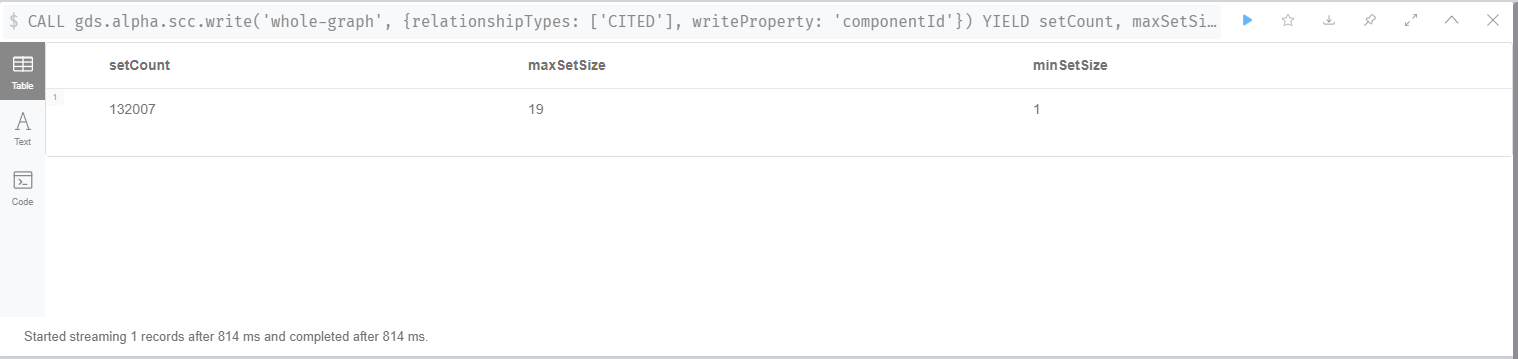
\includegraphics[scale=0.5]{q15.PNG}}
    \caption{Résultat de l'algorithme de recherche des composantes connexes}
\end{figure}

\textbf{Le graphe comporte donc 132007 composantes connexes dont leur taille minimale est 1 et leur taille maximale et 19.}
\item 
Maintenant que les composantes connexes ont été définies, on parcourt alors le graphe et on trie les noeuds en fonction de l'id componentId à laquelle ils appartiennent. On retourne alors le titre des noeuds faisant partie de chaque composante connexe avec la requête suivante :
\begin{lstlisting}
MATCH (n:Article) RETURN n.componentId,count(n.componentId),collect(n.title) ORDER BY count(n.componentId) DESC
\end{lstlisting}
et on obtient les résultats suivants :
\begin{figure}[H]
    \centerline{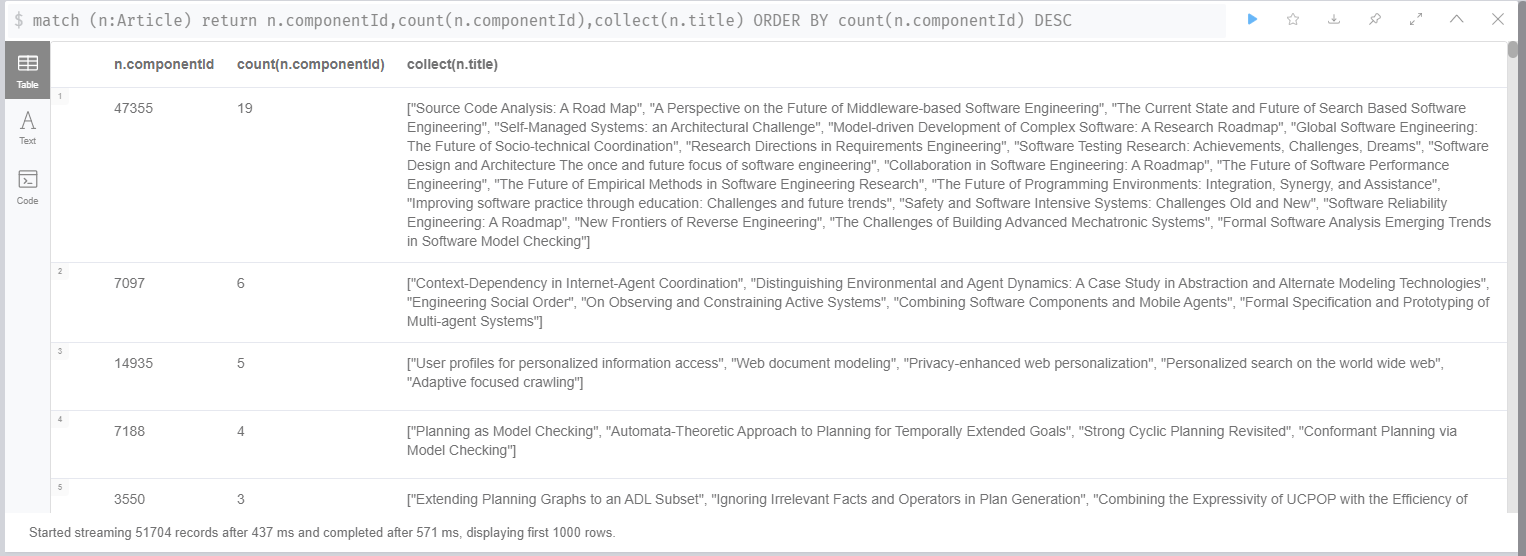
\includegraphics[scale=0.5]{q16.PNG}}
    \caption{Détail de la composition des composantes connexes}
\end{figure}
\item 
On reprend la requête précédente et on limite l'affichage aux 3 premières composantes connexes :
\begin{lstlisting}
MATCH (n:Article) RETURN n.componentId,count(n.componentId) ORDER BY count(n.componentId) DESC LIMIT 3
\end{lstlisting}
puis avec les \textbf{componentId} obtenus, on visualise les noeuds faisant partie de ces composantes connexes avec la requête suivante :
\begin{lstlisting}
MATCH (n:Article) WHERE n.componentId in [47355,7097,14935] RETURN n
\end{lstlisting}
On obtient alors le résultat suivant :
\begin{figure}[H]
    \centerline{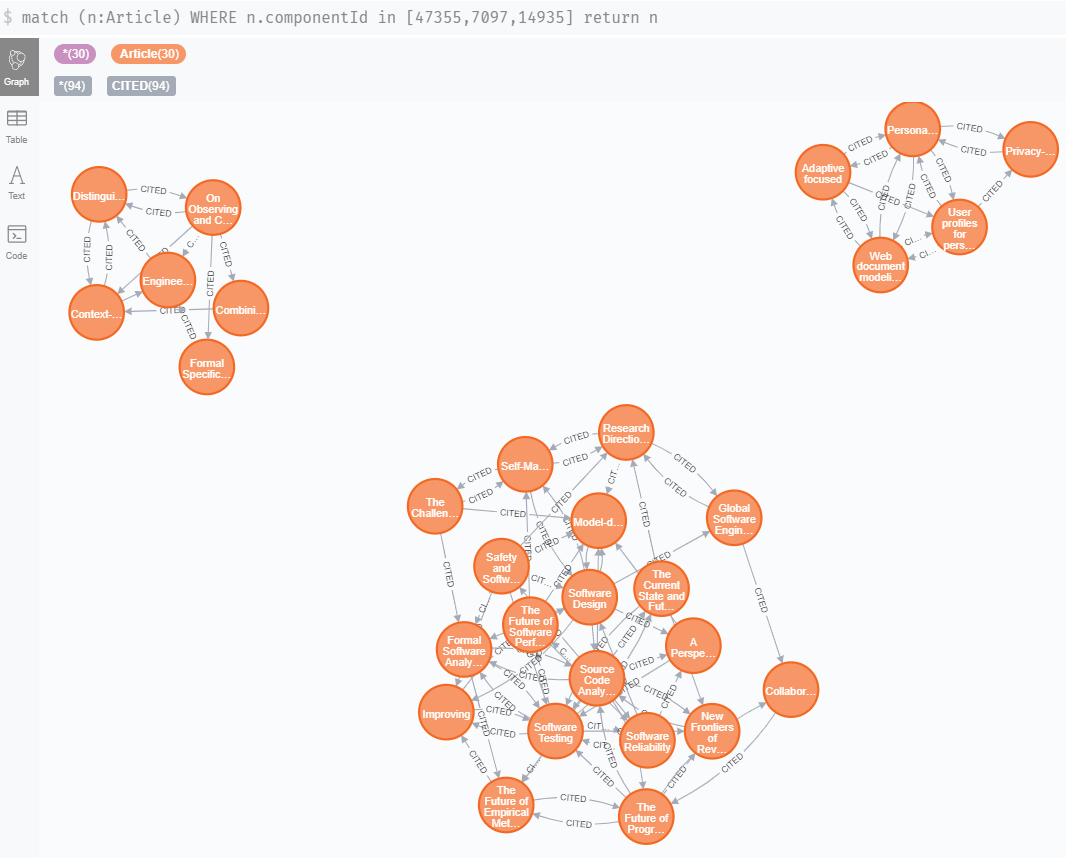
\includegraphics[scale=0.7]{q17b.PNG}}
    \caption{Composantes connexes les plus grandes}
\end{figure}
\item 
On calcule ensuite pour chaque composante connexe la densité de publication en comptant le nombre d'articles publiés par les auteurs de la composante connexe et le nombre d'auteurs de la composante connexe avec la requête suivante :
\begin{lstlisting}
MATCH (n:Article)-[:AUTHOR]->(a:Author) 
RETURN n.componentId,sum(size([(a)<-[:AUTHOR]-(s) | s.title]))*1.0/count(n.componentId) as densite
\end{lstlisting}
On obtient alors les résultats suivants :
\begin{figure}[H]
    \centerline{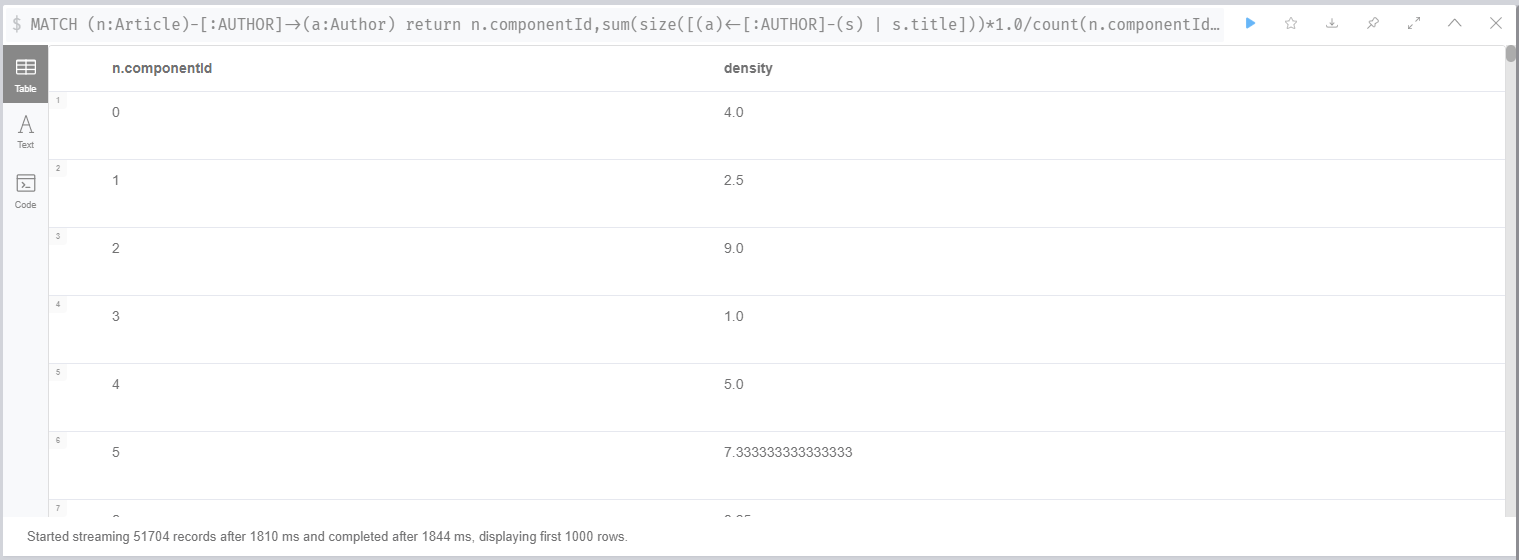
\includegraphics[scale=0.5]{q18.PNG}}
    \caption{Calcul de la densité de publication de chaque composante connexe}
\end{figure}
\br On multiplie le nombre d'articles publiés par les auteurs de la composante connexe par 1.0 pour que l'on obtienne à la fin un résultat sous forme de flottant et non d'entier (car ce serait alors une division entière). \eb
\item 
À partir de la requête précédente, il suffit de trier selon la colonne density et de limiter l'affichage aux 3 composantes avec la plus forte densité :
\begin{lstlisting}
MATCH (n:Article)-[:AUTHOR]->(a:Author) 
RETURN n.componentId,sum(size([(a)<-[:AUTHOR]-(s) | s.title]))*1.0/count(n.componentId) as densite 
ORDER BY densite DESC LIMIT 3
\end{lstlisting}
On obtient alors :
\begin{figure}[H]
    \centerline{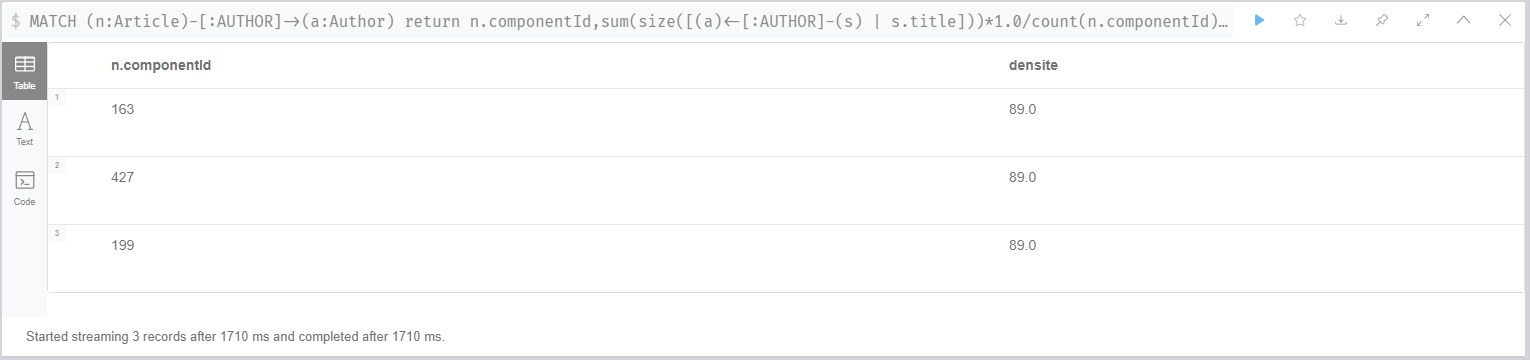
\includegraphics[scale=0.5]{q19.PNG}}
    \caption{Composantes connexes les plus denses en matière de publication}
\end{figure}
\item 
Pour appliquer l'algorithme Louvain, on commence par ajouter une propriété de poids \texttt{weight=1} aux relations de type CO\_AUTHOR :
\begin{lstlisting}
MATCH (a)-[t:CO_AUTHOR]->(b) SET t.weight=1 RETURN type(t)
\end{lstlisting}
Ensuite, on applique l'algorithme Louvain de détection des communautés et on obtient les clusters d'auteurs qui publient ensemble, avec leur id. La requête prend la forme suivante :
\begin{lstlisting}
CALL gds.louvain.stream('whole-graph', { relationshipTypes: ['CO_AUTHOR'] }) 
YIELD nodeId, communityId, intermediateCommunityIds
RETURN collect(gds.util.asNode(nodeId).name) AS name, communityId
ORDER BY size(name) DESC
\end{lstlisting}

Le résultat obtenu se trouve à la page suivante, figure 9. D'après cette figure, la vitesse d'exécution de l'algorithme Louvain est de 5,849 s. Le calcul des composantes connexes effectué à la question 15 a pris quant à lui 814 ms. On conclut donc que l'algorithme Louvain de détection des comunnautés est plus lent que l'algorithme de recherche des composantes connexes. De plus, les résultats ne semblent pas être comparables,notamment en termes de taille de composantes connexes versus la taille des clusters d'auteurs...
\begin{landscape}
\begin{figure}[!p]
    \centerline{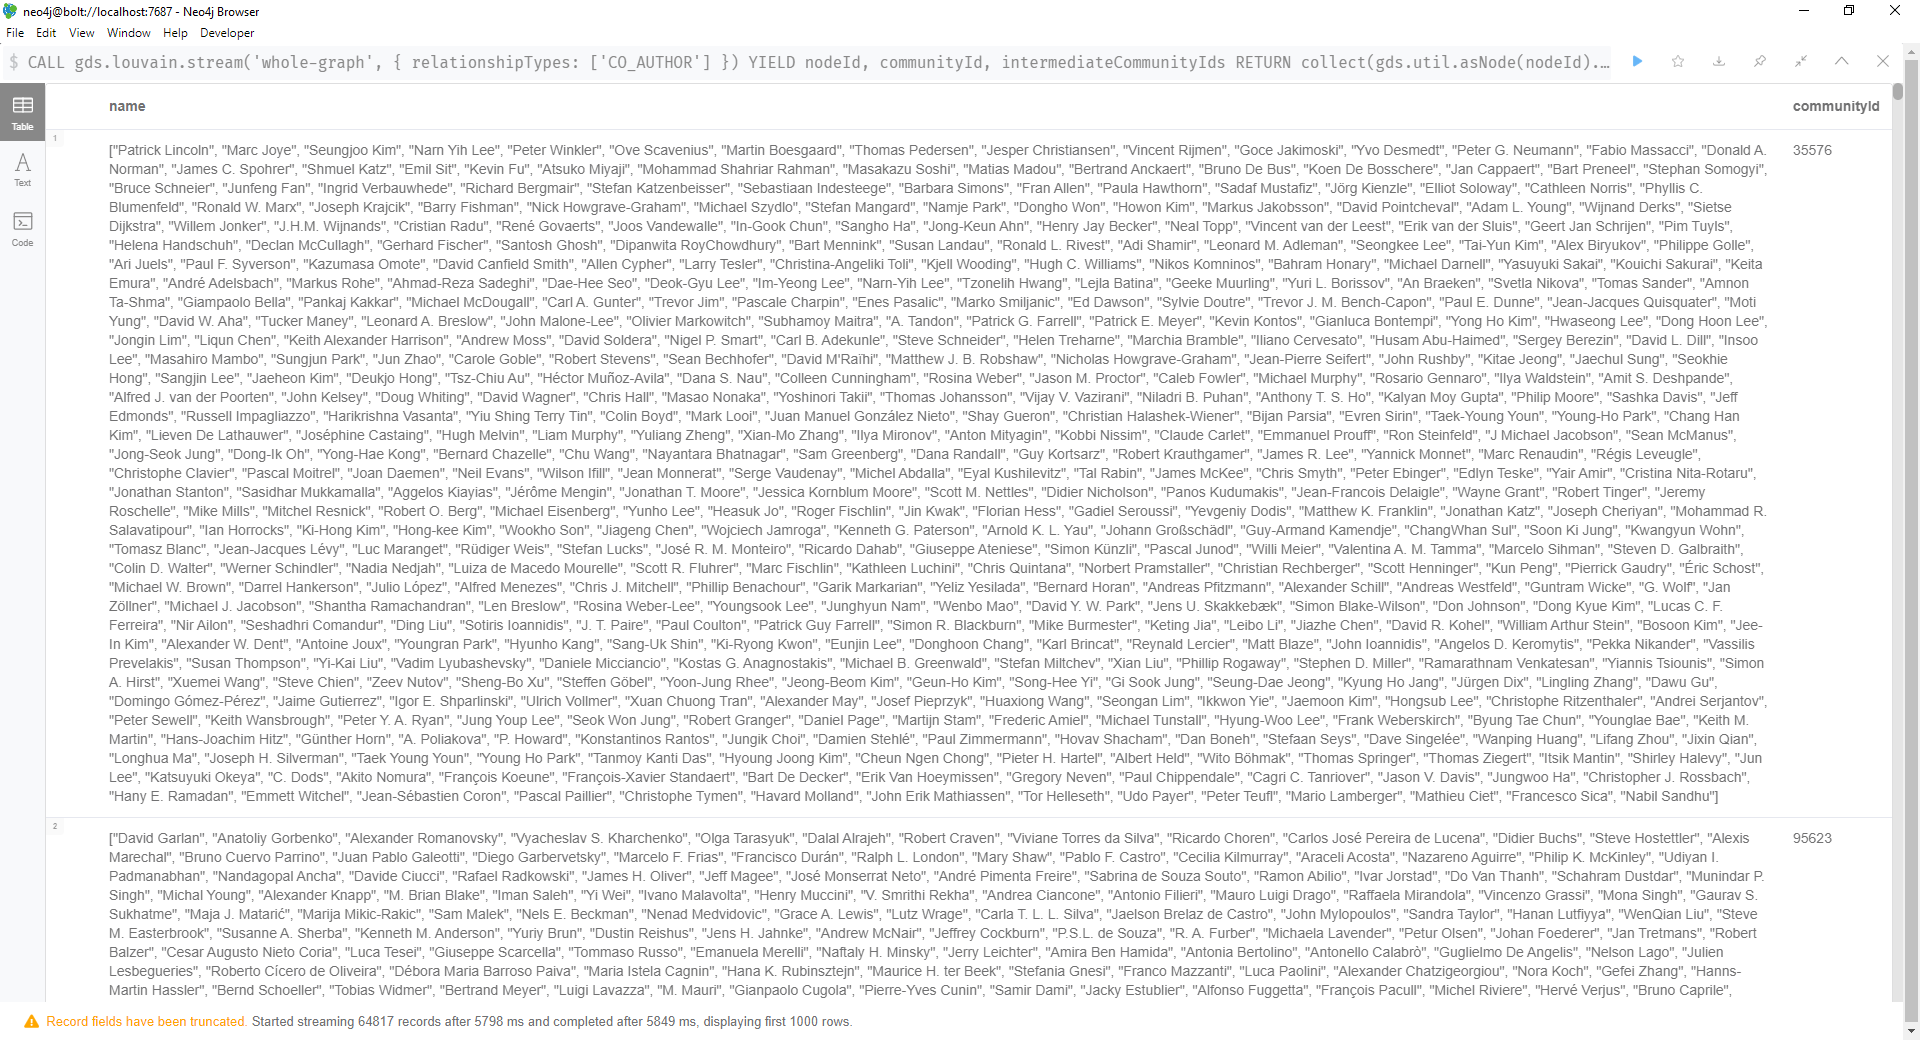
\includegraphics[scale=0.5]{q20.PNG}}
    \caption{Clusters d'auteurs publiant ensemble}
\end{figure}
\end{landscape}
\end{enumerate}
\end{document}

